\documentclass[a4paper,10pt]{article}
\usepackage[utf8]{inputenc}
\usepackage[T1]{fontenc}
\usepackage[left=0pt, right=0pt, top=0pt, bottom=0pt]{geometry}
\usepackage{tikz}
\usepackage{xcolor}
\usepackage{graphicx}
\usepackage{enumitem}
\usepackage{hyperref}
\usepackage{lmodern}
\usepackage{calc}
\renewcommand{\familydefault}{\sfdefault}

% Colors
\definecolor{SidebarColor}{HTML}{F4F4F4}
\definecolor{HeaderColor}{HTML}{758525} % Olive green from image
\definecolor{DarkText}{HTML}{1A1A1A}
\definecolor{LightText}{HTML}{4A4A4A}
\definecolor{GrayText}{HTML}{666666}

\begin{document}
\pagestyle{empty}

% Backgrounds
\begin{tikzpicture}[remember picture, overlay]
    % Left Gray Sidebar
    \fill[SidebarColor] (current page.north west) rectangle ([xshift=7cm]current page.south west);

    % Header Green Banner with a slight slant
    % Top rectangle part
    \fill[HeaderColor] (current page.north west) rectangle ([yshift=-2.8cm]current page.north east);
    % Slanted part
    \fill[HeaderColor] ([yshift=-2.8cm]current page.north west) -- ([yshift=-2.8cm]current page.north east) -- ([yshift=-3.8cm]current page.north east) -- ([yshift=-2.3cm]current page.north west) -- cycle;
    
    % A slight accent line under the slant
    \draw[white, line width=2mm] ([yshift=-2.85cm]current page.north west) -- ([yshift=-3.85cm]current page.north east);

    % Name in header
    \node[anchor=west, text=white, inner sep=0pt] at ([xshift=7.5cm, yshift=-1.8cm]current page.north west) {\fontsize{38}{45}\selectfont \textbf{ARYAN MAURYA}};

    % Profile Picture
    % Clipped circle at the intersection of sidebar and header
    \node[circle, draw=SidebarColor, line width=3mm, fill=white, minimum size=5cm, anchor=center, path picture={
        \node at (path picture bounding box.center) {
            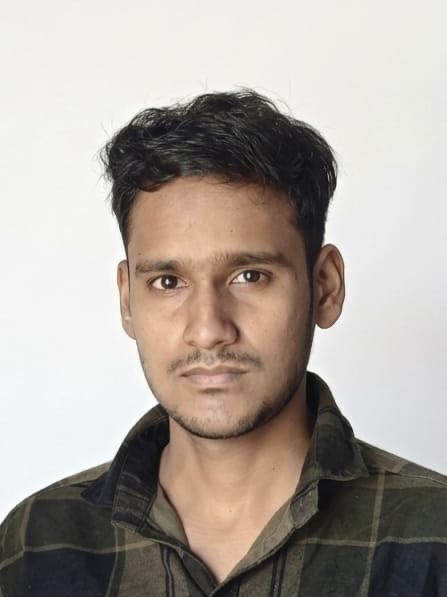
\includegraphics[height=5cm]{profile_photo.png}
        };
    }] at ([xshift=3.5cm, yshift=-1.8cm]current page.north west) {};

\end{tikzpicture}

% Main Content Layout
\vspace*{4.2cm}

\begin{minipage}[t]{7cm}
    \vspace{0pt}
    \hspace*{0.8cm}\begin{minipage}{5.4cm}
        \color{DarkText}
        \large \textbf{CONTACT} \\
        \normalsize
        \vspace{0.1cm}
        \begin{tabular}{@{}l@{\hspace{0.2cm}}l@{}}
            \textbf{Email:} & \href{mailto:aryannsv@gmail.com}{aryannsv@gmail.com} \\
            \textbf{LinkedIn:} & \href{https://linkedin.com/in/aryan-maurya-vns}{aryan-maurya-vns} \\
            \textbf{GitHub:} & \href{https://github.com/aryanRN2}{aryanRN2} \\
            \textbf{LeetCode:} & 200+ Problems Solved \\
            \textbf{Location:} & Varanasi, India
        \end{tabular}
        
        \vspace{0.6cm}
        \large \textbf{KEY SKILLS} \\
        \normalsize
        \vspace{0.1cm}
        \begin{itemize}[leftmargin=*, noitemsep, label={\color{DarkText}\textbullet}]
            \color{LightText}
            \item Agentic AI \& Machine Learning
            \item Fullstack Java Development
            \item Python, JS, TypeScript, SQL
            \item Next.js, React, HTML/CSS
            \item GCP, Vercel, Kubernetes
            \item Database Mgt (PostgreSQL)
            \item Git/GitHub
        \end{itemize}

        \vspace{0.6cm}
        \large \textbf{CERTIFICATIONS} \\
        \normalsize
        \vspace{0.1cm}
        \begin{itemize}[leftmargin=*, noitemsep, label={\color{DarkText}\textbullet}]
            \color{LightText}
            \item Google Data Analytics
            \item Classical ML (IIT Guwahati)
            \item Cloud Computing (IIT Madras)
            \item Machine Learning Specialization (DeepLearning.AI)
            \item LangChain (DeepLearning.AI)
            \item SWE Intern (HackerRank)
        \end{itemize}
        
        \vspace{0.6cm}
        \large \textbf{EDUCATION} \\
        \normalsize
        \vspace{0.1cm}
        \textbf{Banaras Hindu University (BHU)}\\
        \textcolor{GrayText}{BS in Mathematics}\\
        \textcolor{GrayText}{2023 - Present}\\[0.2cm]
        \textbf{IIT Madras (Online)}\\
        \textcolor{GrayText}{BS in Data Science}\\
        \textcolor{GrayText}{2023 - Present}
    \end{minipage}
\end{minipage}%
\hspace*{0.6cm}%
\begin{minipage}[t]{12.2cm}
    \vspace{0pt}
    \begin{center}
        \Large\textbf{ABOUT ME}
    \end{center}
    \vspace{0.1cm}
    
    \begin{center}
        \textbf{Software Engineer and Data Scientist with expertise in full-stack web development and scalable machine learning infrastructure}
    \end{center}
    \vspace{0.1cm}
    
    \textcolor{LightText}{\small Passionate about automating model training pipelines, streamlining feature stores, configuring Kubernetes clusters, and establishing end-to-end MLOps lifecycles. Experienced in designing AI-powered platforms, comprehensive digital libraries, and advanced data-driven web applications using modern technologies like Next.js, Python, PostgreSQL, and GCP.}
    
    \vspace{0.3cm}
    \hrule
    \vspace{0.3cm}
    
    \Large\textbf{PROJECTS}
    \vspace{0.2cm}
    \normalsize
    
    \textbf{SciQB Platform} \hfill \textcolor{GrayText}{2026}\\
    \textcolor{GrayText}{\href{https://sciqb.com}{sciqb.com} $|$ Node.js, JS, Tailwind CSS, Backblaze B2}\\
    \begin{itemize}[leftmargin=*, noitemsep, topsep=0pt, label={\color{DarkText}\textbullet}]
        \color{LightText}\small
        \item \textbf{Full-Stack Development:} Engineered a high-fidelity educational assessment platform serving thousands of university students with mock exams, official syllabi, and transcribed previous year question papers.
        \item \textbf{AI Integration:} Integrated Large Language Models (LLMs) via secure proxies (NVIDIA, HuggingFace) to act as an on-demand intelligent tutor, dynamically explaining complex questions and answers to students.
        \item \textbf{Backend Security \& Architecture:} Built a custom Node.js server featuring a Backblaze B2 integration that generates signed URLs to protect private PDF assets from unauthorized direct downloads.
        \item \textbf{Data Encryption:} Developed an API endpoint with custom XOR encryption to securely deliver over 730+ LaTeX-based question papers (93,000+ lines of code) across 10 university departments to the client side.
        \item \textbf{Modern Frontend:} Designed a responsive, accessible user interface using Tailwind CSS and Vanilla JavaScript, implementing modern design principles like glassmorphism and micro-animations to enhance user engagement.
        \item \textbf{Rate Limiting \& Optimization:} Implemented custom IP-based rate limiting on sensitive API endpoints to prevent abuse and ensure high availability of the assessment engine.
    \end{itemize}
    \vspace{0.3cm}

    \textbf{VRS Digital Library Portal} \hfill \textcolor{GrayText}{2026}\\
    \textcolor{GrayText}{Flask, PostgreSQL, JavaScript, Vercel}\\
    \begin{itemize}[leftmargin=*, noitemsep, topsep=0pt, label={\color{DarkText}\textbullet}]
        \color{LightText}\small
        \item Built a serverless seat allotment platform managing real-time reservations, financial audits, and user memberships.
        \item Designed an interactive seat matrix with automated shift-conflict resolution to guarantee data integrity and prevent double-bookings.
        \item Automated user communications by integrating the WhatsApp Cloud API for instant credential and receipt delivery.
        \item Implemented dynamic PDF receipt generation (ReportLab) and Excel financial data exports for administrative auditing. 
    \end{itemize}
    \vspace{0.3cm}

    \textbf{Mini Projects} \hfill \textcolor{GrayText}{2025 - 2026}\\
    \textcolor{GrayText}{Python, LLMs, NLP, APIs}\\
    \begin{itemize}[leftmargin=*, noitemsep, topsep=0pt, label={\color{DarkText}\textbullet}]
        \color{LightText}\small
        \item \textbf{Handwritten to LaTeX:} Developed a machine learning vision pipeline that accurately interprets handwritten mathematical equations and automatically generates perfectly formatted LaTeX code.
        \item \textbf{Intelligent AI Chatbot:} Built a conversational AI agent capable of context-aware responses, reasoning, and answering user queries using advanced Natural Language Processing and LLM APIs.
    \end{itemize}
    
\end{minipage}

\end{document}
